\documentclass{article}
\usepackage[utf8]{inputenc}
\usepackage[T1]{fontenc}
\usepackage{graphicx}
\usepackage{hyperref}
\usepackage{geometry}
\geometry{margin=1in}

\title{HUGHES (John}
\date{Encyclopaedia Britannica (1771)}

\begin{document}
\maketitle

\section*{Historical source}
\textbf{Entry ID:} \texttt{entry-hughes-john-1327} \\
\textbf{Volume ID:} 149981670 \\
\textbf{Character Count:} 1106

\subsection*{Extracted Text}
HUGHES (John), an ingenious and polite wri-
ter, was born in 1677. In the earliest parts of his
youish, he continued the difference, poetry, drawing,
and minds, in each of which he by team made a con-
fidercable progress() but followed thoof and his other
fluides only as regarded amendments, except frequent
containment on account of his illust of health. The
land Chanelhoe Cowper made hint forecerty for the
commitons of the peace, not his knowledge, and
illinguished him with singular marks of his clients.
He contained in the farm employment under the end
of Meschelek, and had it to the day of his death,
which happened in 1719, the very light in which his
tragedy, entitled \_The large of Damar, was first ac-\_
ing. He was then ... He realized Pontoredley
dialogues of the dead, Vertact's evolutions of Portu-
gal, and the latter of Abrilad and Dolits. He gave
very accurate edition of species's works, with his
life, a gloffary, and remarks; and wrote several papers
in the Father, Speichere, and Grandians Mr Duno-
combo, who married his father, collected his poems
and days in a vols 12mo, in 735.



\section*{Source record}
\begin{itemize}
\item \textbf{Dataset:} \texttt{NationalLibraryOfScotland/encyclopaedia\_britannica\_illustrated}
\item \textbf{Dataset Revision:} \texttt{309f765b1ecc83e0a7f7762e44b4a927a7555443}
\item \textbf{Page ID:} \texttt{britannica:309f765b1ecc83e0a7f7762e44b4a927a7555443:train:1327} \\
  \textbf{Filename:} \texttt{page-1327-7d41b1db21d5.jpg} \\
  \textbf{Row Index:} 1327 \\
  \textbf{SHA256:} \texttt{7d41b1db21d5e291...}
\end{itemize}

\begin{figure}[h]
\centering
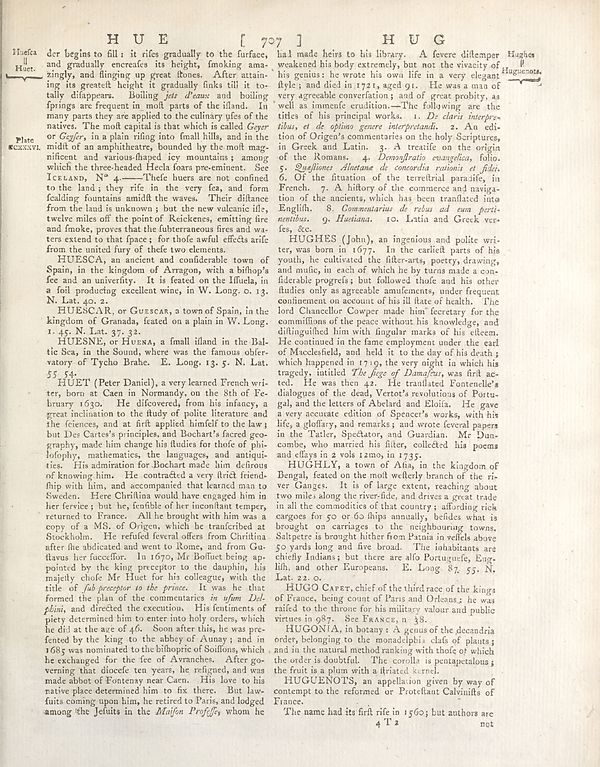
\includegraphics[width=0.85\textwidth]{../scans/page-1327-7d41b1db21d5.jpg}
\caption*{Source scan: \texttt{page-1327-7d41b1db21d5.jpg}}
\end{figure}

\end{document}
